\documentclass[a4paper, 11pt]{article}

\voffset -0cm
\hoffset 0.0cm
\textheight 23cm
\textwidth 16cm
\topmargin 0.0cm
\oddsidemargin 0.0cm
\evensidemargin 0.0cm

\usepackage{epsfig}
\usepackage{setspace}
\usepackage{fancyheadings}
\usepackage{amsmath}
\usepackage{amssymb}
\usepackage{graphicx}
\usepackage{url}

\title{}
\author{}
\date{}

\begin{document}

\begin{center}
	\LARGE \textbf{TP6: Rasterization of triangles}
\end{center}

\bigskip
\par The process of rasterization converts a vector image (or a set of analytical shapes) into a set of pixels (call fragments in Computer Graphics).
We will here implement a triangle rasterizer using the Bresenham digitization of segments.

\paragraph{Question} Implement the Bresenham's digitization of an Euclidean segment defined by the origin and the point (in integer coordinates).

\section*{Standard Algorithm}

The standard algorithm for rasterizing triangles uses the fact that their exists two easy cases to draw: a flat bottom and a flat top triangle (see Figure \ref{fig:triangles}).
The idea of the algorithm is to traverse both legs step by step in the y-direction and draw a straight horizontal line between both endpoints.

\paragraph{Question} Can you infer the algorithm for an arbitrary triangle ($V_1,V_2,V_3$) ?

\begin{figure}
  \centering
  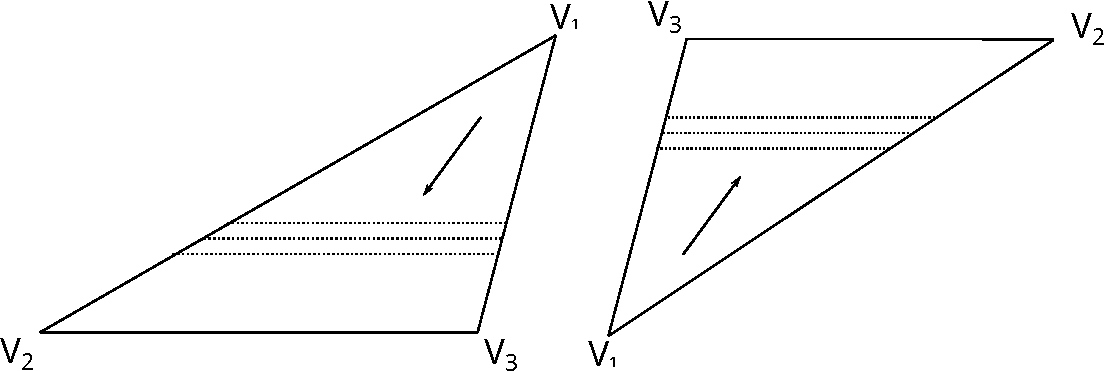
\includegraphics[width=\textwidth]{triangles}
  \caption{The bottom flat triangle on the left, and the top flat one on the right. Lines are drawn parallel to segment $V_2,V_3$.}
  \label{fig:triangles}
\end{figure}

\vspace{5mm}
\noindent The idea is now to use the Bresenham algorithm to draw the triangle lines, and connect each fragments that are at the same y-level with a straight line.

\paragraph{Question} Implement the rasterization algorithm of one triangle.

\section*{$z$-buffer}

We now suppose that we have $N$ triangles and for each triangle a $z$ position (where $z=0$ means that the triangle is on the screen).

\paragraph{Question} Implement a rendering algorithm of $N$ triangles using a $z$-buffer by sorting them. Display a graph showing the speed of you algorithm regarding the number of input triangles.

\paragraph{Question} Implement another rendering algorithm of $N$ triangles using the $z$-buffer: this time, don't sort the input triangles but instead for each fragment generated by the rasterization algorithm
keep in mind the $z$ coordinate of of the fragment and render it only if its closer to the screen than the previous one. It it faster than the previous algorithm ?

\vspace{5mm}
\noindent We suppose now that each triangle has a $z$ coordinate for each of its vertice (ie. that they lie in $\mathbb{R}^3$) and that their projection fits within the screen (see Figure \ref{fig:zbuffer}).

\paragraph{Question} Adapt the last algorithm to render $N$ triangles on the screen. You will have to interpolate the $z$ coordinates for each fragment computed during the rasterization.

\begin{figure}
  \centering
  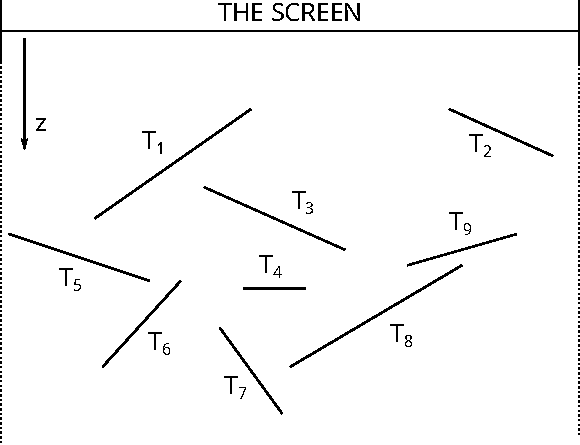
\includegraphics[width=\textwidth]{zbuffer}
  \caption{A top view of the set of triangles to rasterize. Each triangle has a different $z$-coordinate for each of its vertice.}
  \label{fig:zbuffer}
\end{figure}

\end{document}
